\chapter{Literatūras apskats}

Ir aprakstītas vairākas metodes, lai veiktu cilvēku plūsmu analīzi attēlos un video fragmentos \cite{brostow2006unsupervised,chen2013cumulative,ge2009marked,chen2015person,lempitsky2010learning}. Vispārīgi, pirmie pētījumi tika vērsti uz detektēšanas veida izvēli un vai problēmu var risināt izmantojot segmentācijas metodes \cite{tu2008unified}. Šīs metodes nelabvēlīgi ietekmēja objektu nostāšanās vienam aiz otra, objektu pazušana un nekārtīgs (pārblīvēts TODO pārbaudīt tulkojumu (high clutter background)) fons attēlos. Jaunākos risinājumus var vispārīgi sadalīt trīs kategorijās: risinājumi, kas balstīti uz regresiju, risinājumi, kas balstīti uz pūļa blīvuma novērtējumu un risinājumi, kas balstīti uz konvolūcijas neironu tīkliem. 

\subsubsection{Risinājumi, kas balstīti uz regresiju}
Lai novērstu objektu paslēpšanos attēlā un pārblīvēta fona problēmas, pētnieki mēģināja skaitīt cilvēkus izmantojot regresiju. Parasti, regresija šādos risinājumos tiek veikta starp dažādām attēla īpašībām un objektu skaitu. Šāds risinājums sadala attēlu vairākos mazākos attēlos un katram šim mazajam attēlam tiek veikta aptuvenā skaita noteikšana izmantojot segmentācijas metodes. Lai noteiktu kopējo cilvēku skaitu attēlā, ir jāsaskaita katra mazā attēla aptuvenie novērtējumi. Lai apmācītu šādu sistēmu, pirmais no attēla apstrādes posmiem ir atmest attēla fonu un veikt \textit{ground-truth} novērtējumu, kas nozīmē, ka tiek manuāli izskaitīts cilvēku skaits katrā sadalītajā attēlā  \cite{chan2009bayesian,ryan2009crowd,chen2012feature}.

Šāda pieeja tika izveidota, pieņemot, ka dotajai cilvēku skaitīšanas sistēmai būtu vieglāk novērtēt cilvēku daudzumu katrā grupā atsevišķi, nevis novērtēt cilvēku daudzumu visam pūlim vienlaikus. Pieņemot, ka attēlā ir pūlis ar 20 cilvēkiem, šo pūli var sadalīt divās lielās grupās vai arī desmit pāros. Ņemot šādu attēlu vispārīgi, šāds pūļa sadalījums var nebūt tik skaidri novērtējams, jo attēlam vispārīgi būtu daudz vairāk atšķirīgu īpašību. Eksistējošas metodes, kas izmanto visu attēlu no attēla iegūst daudz vairāk īpašību, kas nozīmē, ka ir nepieciešami vairāk apmācības datu \cite{chan2008privacy}. Pētot citus rakstus var secināt, ka regresijas metodes parasti sastāv no divām lielām komponentēm: zema līmeņa īpašību iegūšanas un regresijas modeļa implementēšanas \cite{xiong2017spatiotemporal}. 

\subsubsection{Risinājumi, kas balstīti uz pūļa blīvuma novērtējumu}
Lai gan pūļu skaitīšanas risinājumi, kas balstīti uz regresiju veiksmīgi tika galā ar objektu pārklāšanās un pārblīvētā fona problēmām, tika palaista garām svarīga telpiska informācija, jo regresija tika izmantota uz lokālajām īpašībām (katra sadalītā attēla īpašībām atsevišķi). Pētījumā \cite{lempitsky2010learning} tiek piedāvāts jauns veids kā iemācīties lineāras attiecības starp sadalīto attēlu īpašībām un attiecīgās objektu blīvuma kartes izmantojot regresiju. Novērojot, ka iemācīties lineāras attiecības ir sarežģīts uzdevums, tika izveidots risinājums, kas piedāvā iemācīties nelineāras attiecības starp sadalīto attēlu īpašībām un objektu blīvuma kartēm izmantojot nejaušo mežu ietvaru (no angļu val. \textit{random forest framework}) \cite{pham2015count}. Vairāki mūsdienu risinājumi piedāvā metodes, kas balstās uz blīvuma karšu regresiju \cite{wang2016fast,xia2016block}. 

\subsubsection{Risinājumi, kas balstīti uz konvolūcijas neironu tīkliem}
Tā kā mūsdienās klasifikācijā un atpazīšanas uzdevumu risināšanā ļoti veiksmīgi darbojas uz konvolūcijas neironu tīkliem balstītas metodes. Pētnieki ir izveidojuši CNN, ar mērķi veikt pūļa skaitīšanu un blīvuma novērtējumu \cite{wang2015deep,shang2016end,walach2016learning}. Pretēji jau eksistējošajām metodēm, kas pūļa skaitu novērtē izmantojot attēla sadalīšanas metodes, Šangs \cite{shang2016end} piedāvā metodi, kas veic novērtējumu izmantojot CNN. Šī metode novērtējumu veic paralēli skaitot cilvēkus gan globālajā kontekstā, gan lokālajā kontekstā. Žangs \cite{zhang2016single} piedāvāja daudz-kolonnu arhitektūru, kas izgūst īpašības dažādos mērogos. Līdzīgi šai metodei, tika izveidots skaitīšanas modelis, kas veica novērtējumu pūļa blīvuma kartēm, ko nosauca par \textit{Hydra CNN} \cite{onoro2016towards}. Pētnieks Mardsens \cite{marsden2017resnetcrowd} pētīja pilnīgos konvolūciju neironu tīklus un vairākuzdevumu (no ang. val. \textit{multi-task}) apmācību, kuru apvienojot veica cilvēku skaitīšanu. Minētie vairākuzdevumu apmācības un daudz-kolonnu risinājumi ir sasnieguši labus rezultātus, uzrādot salīdzinoši zemu skaitīšanas kļūdu. Balstoties uz minētajiem risinājumiem var izdarīt sekojošus secinājumus \cite{sindagi2017generating}:
\begin{itemize}
	\item Šīs metodes neietver kontekstuālu informāciju, kas ir svarīgi, lai iegūtu labākus rezultātus;
	\item Lai gan eksistējošie risinājumi izmanto regresiju ar pūļa blīvuma kartēm, šie risinājumi ir vairāk balstīti uz skaitīšanas kļūdas samazināšanu, nevis blīvuma karšu kvalitātes uzlabošanu;
\end{itemize}
\newpage
Šī darba ietvaros tiks veikta skaitīšana pēc detektēšanas. Tas nozīmē, ka tiks izmantots atsevišķs objektu detektēšanas risinājums, kas objektus lokalizēs pēc konvolūciju neironu tīkla klasifikācijas atrastās klases. Kad lokalizētas visas objekta instances, skaitīšanas uzdevums paliek elementārs. Taču objektu detektēšanas problēmām nav atrasti risinājumi, kas strādā nevainojami, it īpaši, ja vairākas objektu instances attēlā pārklājas. Vienkāršākie objektu detektēšanas risinājumi balstās uz divām operācijām: izveidot reālu vērtību pārliecības (no angļu val. \textit{confidence}) karti un izmantojot šo karti, tiek meklētas augstās vērtības, kas atbilst individuālām objektu instancēm. Vairākas metodes pieņem, ka attēlos ir vairāki vienādi objekti un tos vienu no otra var atšķirt izmantojot \textit{Monte-Carlo} procesu \cite{descombes2009object}, morfoloģisko analīzi \cite{selinummi2005software} un variāciju optimizāciju \cite{nath2006cell}. Mūsdienās, populārākās un precīzākās metodes objektu detektēšanai ir \textit{YOLO} (\textit{You Only Look Once}) \cite{redmon2016you}, \textit{Faster-RCNN} (\textit{Faster Region-Based Convolutional Neural Network}) \cite{ren2015faster} un \textit{SSD} (\textit{Single Shot MultiBox Detector}) \cite{liu2016ssd}.
\subsubsection{YOLO (\textit{You Only Look Once})}
\textit{YOLO} pārveido objektu detektēšanas problēmu par vienkāršas regresijas problēmu, veicot regresiju starp attēla pikseļiem, ierobežojošo logu (no angļu val. \textit{bounding box}) koordinātēm un klašu varbūtībām. Viens konvolūciju neironu tīkls vienlaicīgi veic daudz ierobežojošo logu prognozes un klašu varbūtības šiem logiem. Šādam modelim ir vairākas priekšrocības salīdzinājumā ar citām objektu detektēšanas metodēm: 
\begin{itemize}
	\item Tas ir ļoti ātrs. Tā kā detektēšana tiek pārvērsta par parastu regresijas problēmu, nav nepieciešams sarežģīts vairāku procesu kopums. 
	\item Kad \textit{YOLO} izdara prognozes par attēlu, tiek ņemts viss attēls kopumā. Pretēji slīdošo logu metodēm un uz reģionu minējumiem balstītajām metodēm, \textit{YOLO} sistēma apmācības laikā redz visu attēlu, tādējādi tas ir spējīgs netieši klasēm pievienot to kontekstuālo informāciju.
	\item \textit{YOLO} iemācās vispārējus objektu attēlojumus, kas nozīmē, ka pielietojot šo sistēmu tam nepazīstamiem datiem vai negaidītiem ievades datiem, ir salīdzinoši mazāka iespēja, ka tas kļūdīsies. 
\end{itemize}

\textit{YOLO} detektēšanas sistēma sadala ievades attēlu režģī. Ja objekta centrs trāpās kādā no režģa šūnām, tad šī šūna ir atbildīga par šī objekta detektēšanu. Katra šūna prognozē noteiktu ierobežojošo logu (\textit{bounding boxes}) skaitu, kā arī pārliecības rezultātus (\textit{confidence scores}) šiem logiem. Šie pārliecības rezultāti norāda cik pārliecināta ir sistēma par to ka ierobežojošajos logos ir objekts un cik precīzi ir novietots pats ierobežojošais logs. Pārliecību matemātiski izsaka kā objekta varbūtības un \textit{IoU} (\textit{intersection over union}) reizinājumu. Ja šūnā nav neviena meklētā objekta, tad pārliecības rezultāts būs nulle.

\begin{figure}[h]%
	\centering
	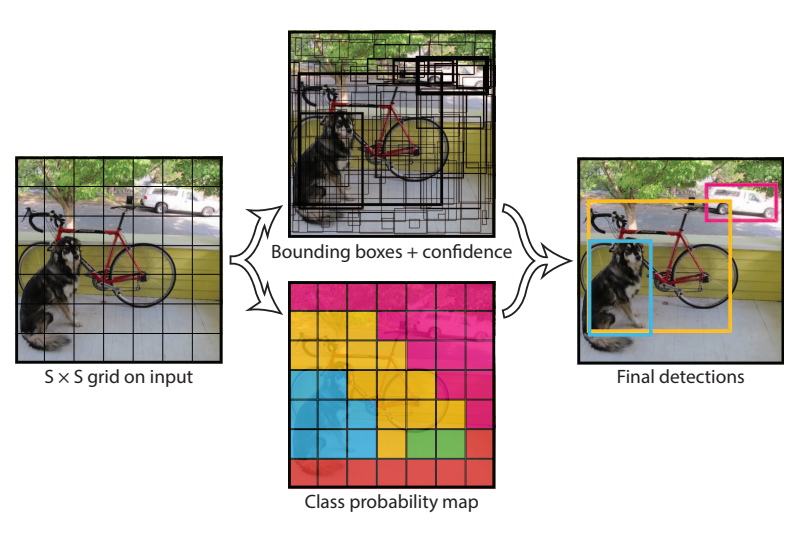
\includegraphics[height=6cm]{images/yolo.png} %
	\caption{\textit{YOLO} modelis \cite{redmon2016you}}%
	\label{fig:example}%
\end{figure}

Katrs ierobežojošais logs satur piecas prognozes: koordinātes, kas norāda loga centru attiecībā pret režģa šūnām, loga augstuma un platuma vērtības un pārliecības vērtību. Katra šūna prognozē nosacītās klašu varbūtības. Neatkarīgi no atrasto ierobežojošo logu skaita, katrai šūnai tiks piešķirta tikai viena klase.

Pētījumā \cite{redmon2016you} minētajai standarta \textit{YOLO} sistēmai ir 24 konvolūcijas slāņi, kam seko 2 pilnīgi savienotie slāņi. Pirmie konvolūcijas slāņi iegūst attēlu īpašības, kamēr pilnīgi savienotie slāņi prognozē objektu varbūtības un koordinātes.

\begin{figure}[h]%
	\centering
	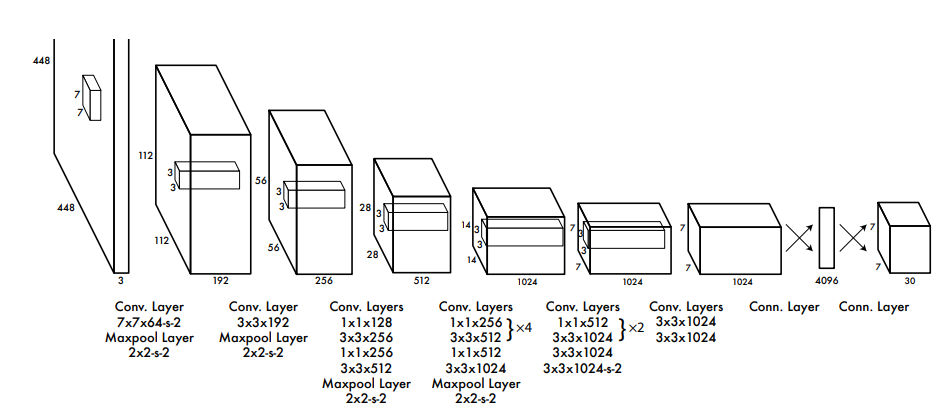
\includegraphics[height=7cm]{images/yoloarch.png} %
	\caption{\textit{YOLO} tīkla arhitektūra \cite{redmon2016you}}%
	\label{fig:example}%
\end{figure}
\newpage
Lai gan \textit{YOLO} ir labs un ātrs risinājums objektu detektēšanā, tam ir savi ierobežojumi:
\begin{itemize}
	\item Šī sistēma uzliek telpiskus limitus ierobežojošo logu prognozēm, jo katra režģa šūna prognozē tikai divus logus un katrai šūnai var piešķirt tikai vienu klasi. Šāds telpisks ierobežojums, limitē cik tuvumā esošus objektus \textit{YOLO} modelis var atrast. Tas nozīmē, ka sistēmai problēmas sagādā mazi objekti, kas atrodas grupās, piemēram, putni.
	\item Līdzīgi kā citas objektu detektēšanas metodes, \textit{YOLO} iemācās veikt ierobežojošo logu prognozes balstoties uz apmācības datiem, kas nozīmē, ja objektu detektēšana jāveic attēliem ar neierastiem izmēriem vai uzstādījumiem, \textit{YOLO} var būt grūti izšķirt objektus šajos attēlos.
	\item Attēlā 2.2 ir redzams, ka tīkla arhitektūrā ir vairāki apvienošanas slāņi (\textit{Maxpool layer}), kas nozīmē, ka ierobežojošo logu prognozēšanā tiek izmantotas salīdzinoši zemas kvalitātes (no angļu val. \textit{coarse}) īpašības. 
	\item Apmācības laikā izmantotā \textit{loss} funkcija pieņem, ka kļūdas mazajos ierobežojošajos logos ir tik pat būtiskas kā kļūdas lielajos logos, kas nav labs risinājums. Mazai kļūdai lielā logā ir maza ietekme, taču tikpat mazai kļūdai mazā logā var būt liela ietekme uz pārliecības rezultātiem. 
\end{itemize}   

\subsubsection{Faster-RCNN (\textit{Faster Region-Based Convolutional Neural Network})}
\textit{Faster-RCNN} ir objektu detektēšanas sistēma, kas sastāv no diviem tīkliem: reģionu piedāvāšanas tīkla (no angļu val. \textit{region proposal network}) jeb RPN, kas veido reģionu priekšlikumus, kurus tālāk piedāvā citam tīklam, kas šiem reģioniem veic objektu detektēšanu. RPN atgriež vairākus logus jeb priekšlikumus, kurus novērtēs klasifikators un regresors, lai noteiktu objektu esamību konkrētajā logā. Tīkls prognozē varbūtību, ka reģionu logs ir fons vai priekšplāns un precizē reģiona loga izmērus. 
